\documentclass[a4paper,12pt]{report}
\usepackage[utf8]{inputenc}
\usepackage[francais]{babel}
\usepackage{fancyhdr}
\usepackage{graphicx}
\usepackage{tikz}
\usetikzlibrary{calc}
\usepackage{listings}
\usepackage{xcolor}
\definecolor{grey}{rgb}{0.9,0.9,0.9}
\usepackage{titlesec}
\usepackage{verbatim}
\usepackage{listings}
\usepackage{textcomp}
\usepackage{hyperref}
\usepackage{longtable}
\usepackage{colortbl}
\usepackage{amssymb}


\frenchbsetup{StandardLists=true}
\newcommand{\marge}{18mm}
\usepackage[left=\marge,right=\marge,top=\marge,bottom=\marge]{geometry}
\pagestyle{fancy}
\setlength{\headheight}{14pt}
\chead{
  \textbf{Binôme :} Douaille Erwan 
    \hspace{2em}
  \textbf{Groupe :} M2 Info IVI}
\renewcommand{\headrulewidth}{1pt}
\linespread{1}
\setlength{\columnseprule}{0.2pt}
\definecolor{javakeyword}{rgb}{0,0,0.5}
\definecolor{javastring}{rgb}{0,0.5,0}
\definecolor{javacomment}{rgb}{0.5,0.5,0.5}
\lstdefinestyle{Scilab}{
   language=Scilab, basicstyle=\footnotesize,       % the size of the fonts that are used for the code
  numbers=left,                   % where to put the line-numbers
  numberstyle=\tiny\color{gray},  % the style that is used for the line-numbers
  stepnumber=1,                   % the step between two line-numbers. If it's 1, each line
                                  % will be numbered
  numbersep=5pt,                  % how far the line-numbers are from the code
  backgroundcolor=\color{white},  % choose the background color. You must add \usepackage{color}
  showspaces=false,               % show spaces adding particular underscores
  showstringspaces=false,         % underline spaces within strings
  showtabs=false,                 % show tabs within strings adding particular underscores
  frame=single,                   % adds a frame around the code
  rulecolor=\color{black},        % if not set, the frame-color may be changed on line-breaks within not-black text (e.g. commens (green here))
  tabsize=2,                      % sets default tabsize to 2 spaces
  captionpos=b,                   % sets the caption-position to bottom
  breaklines=true,                % sets automatic line breaking
  breakatwhitespace=false,        % sets if automatic breaks should only happen at whitespace
  title=\lstname,                 % show the filename of files included with \lstinputlisting;
   stringstyle=\color{javastring},
   keywordstyle=\color{javakeyword}\ttfamily\textbf,
   commentstyle=\color{javacomment}\ttfamily\textit
 }
 

\begin{document}



\makeatletter
\begin{titlepage}
\centering
\vspace{-10em}
{\LARGE \textbf{\textsc{Rapport de Projet RVI}}}\\
\vspace{3em}

\includegraphics[scale=0.6]{image/thalassa.png}\\
\vspace{3em}
{\LARGE \textsc{Projet Thalassa: simulation de plongée sous-marine}}\\

\vspace{8em}
Par\\
\vspace{1em}
{\LARGE \@author}\\

\vspace{2em}



\begin{tikzpicture}[remember picture,overlay]

\node [below left,xshift=-1cm, yshift=4cm] at (current page.south east){
\includegraphics[scale=0.6]{image/ustl1.png}};

\end{tikzpicture}
\end{titlepage}
\makeatother

\sloppy

\setcounter{page}{1} 
\newpage

\section*{Introduction}

Après avoir réaliser le \textit{tri-modal} et le \textit{bi-modal} nous allons voir dans ce TP les limites de la méthode de \textit{Otsu}. Nous décrirons la limite de ce modèle grâce à l'image \textit{3$\_$classes$\_$RGB.tif} et nous proposerons une méthode permettant de seuiller des images malgrès les contraintes de la méthode de \textit{Otsu}. Cette méthode est la méthode \textit{PCA}.

\section*{Analyse en composantes principales}

\subsection*{Est-ce que l'algorithme précédent (analyse des histogrammes R et G) permet de segmenter correctement l'image "3$\_$classes$\_$RGB.tif" ? }

Non. 


\begin{figure}[!ht]
	\center	
	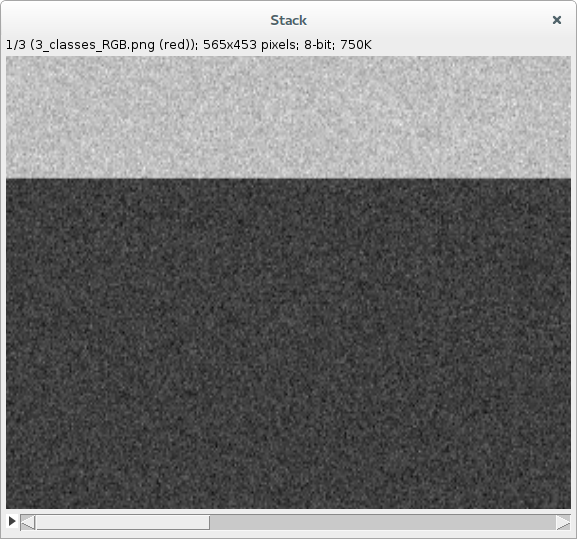
\includegraphics[scale=0.25]{image/stack-1.png}
	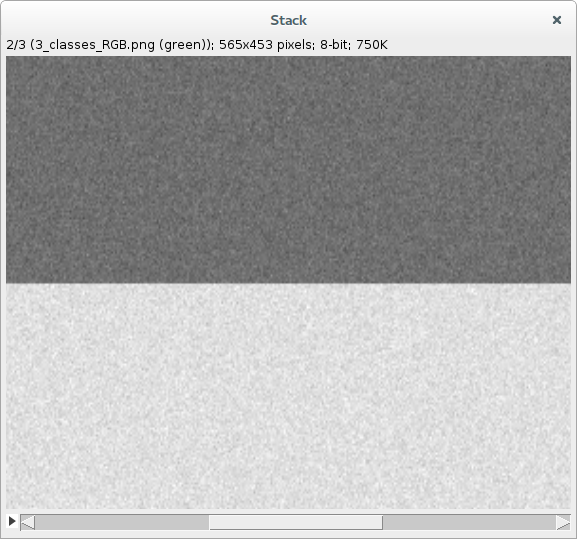
\includegraphics[scale=0.25]{image/stack-2.png}
	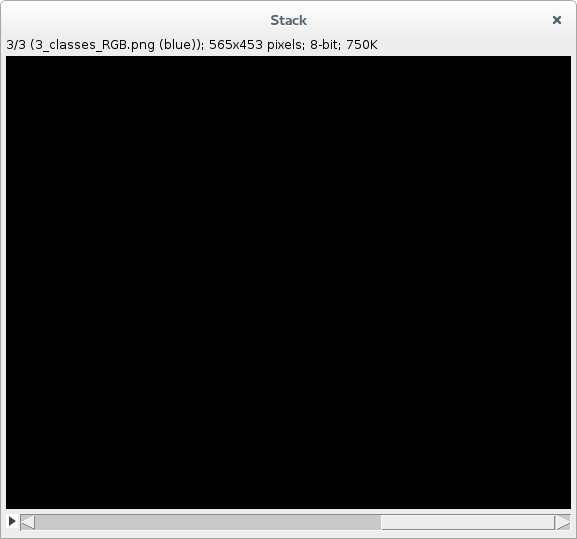
\includegraphics[scale=0.25]{image/stack-3.png}
\end{figure} 

Comme visible sur les composantes RGB de l'image, on ne peut pas appliquer la macro otsu que l'on a réalisé précédemment car on fait déterminer 2 seuils pour la verte et 1 seuil sur la rouge. Trouver 2 seuils sur la verte est impossible. Si on applique un otsu bi-modal sur la composante verte on se retrouve au final avec 4 parties distinctes alors que l'image de base ne posède que 3 parties.

Voici ce qu'on obtiens avec la méthode otsu:

\begin{figure}[!ht]
	\center	
	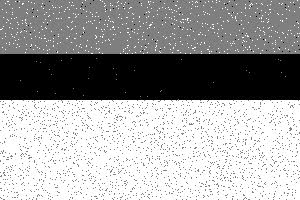
\includegraphics[scale=1]{image/probleme.jpg}
\end{figure} 

On remarque bien que pour la partie grise et blanche la segmentation n'est pas correcte. Ce problème est dûe au non chevauchement des parties claires des composantes rouge et verte.

Chaque composante ne possède pas suffisament d'informations pour déterminer une image correcte.

C'est pour cette raison que nous allons utiliser la méthode PCA (Principal Component Analysis).

\subsection*{Méthode PCA}

La méthode PCA, autrement appelée Transformée de Karhunen-Loève (TKL), permet d'analyser les composantes et de nous fournir une palette de composantes contenant le plus d'informations possibles. Ces composantes sont totallement différente des composantes RGB classiques.

Voici un apercu de ces nouvelles composantes:

\begin{figure}[!ht]
	\center	
	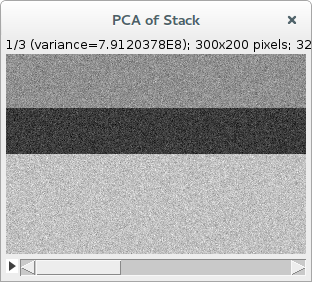
\includegraphics[scale=0.5]{image/pca-stack-1.png}
	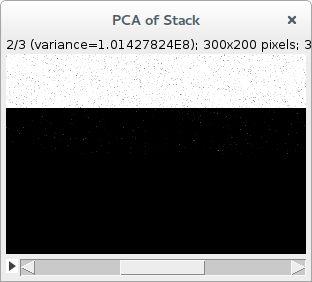
\includegraphics[scale=0.5]{image/pca-stack-2.png}
	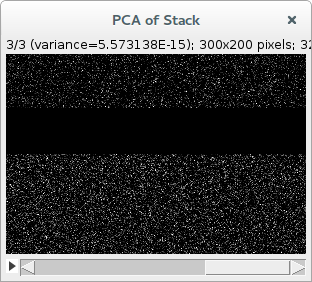
\includegraphics[scale=0.5]{image/pca-stack-3.png}
\end{figure} 

On observe qu'un paramètre nommé variance apparaît. Ce paramètre indique quelle composante possède le plus d'informations. Dans notre exemple, la première à $\sim$7, est celle sur laquelle nous travaillerons. À partir de maintenant nous pouvons appliquer la méthode \textit{Otsu} à cette nouvelle image, voici le résultat:

\begin{figure}[!ht]
	\center	
	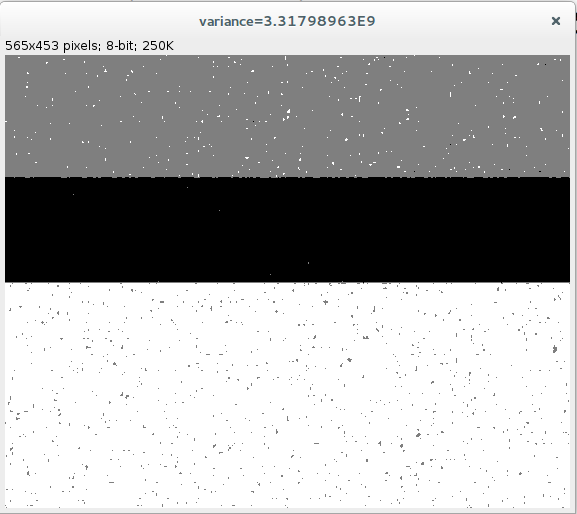
\includegraphics[scale=0.3]{image/final-result.png}
	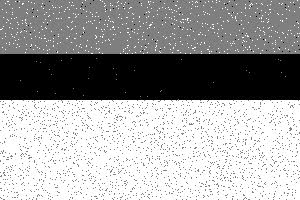
\includegraphics[scale=0.7]{image/probleme.jpg}
\end{figure} 

À gauche notre seuillage obtenue en utilisant l'analyse pas composante principale (PCA) et à droite l'image obtenue en utilisant uniquement la méthode \textit{Otsu}.

On remarque que le seuillage à fonctionner parfaitement et que l'image est maintenant moin bruitée.


\section*{Conclusion}

La méthode \textit{Otsu} comme nous l'avons observé est limitée. Elle ne permet pas de seuiller correctement n'importe quelle image dans le cas ou ses composantes de couleurs deviennent complexes, le mélange dess composantes rouges et vertes dans notre exemple.

Nous avons pu aborder une nouvelle technique qui consiste à utiliser l'analyse par composante primaire avant de segmenter l'image, ce qui a eu pour résultat une image finale moin bruitée.

\end{document}